\section{Devices}
\label{sec:devices}

We had to build prototypes for research purposes and needed to decide which wearables we intend to work with.
Although we wanted to support the widest range of devices that we could, we had to ditch some in order to be able to iterate fast.
In the following section, we will list the advantages and disadvantages of different wearables.
Namely, we evaluated the Apple Watch, the UP and Microsoft Band as well as Android watches.

\begin{figure}[H]
	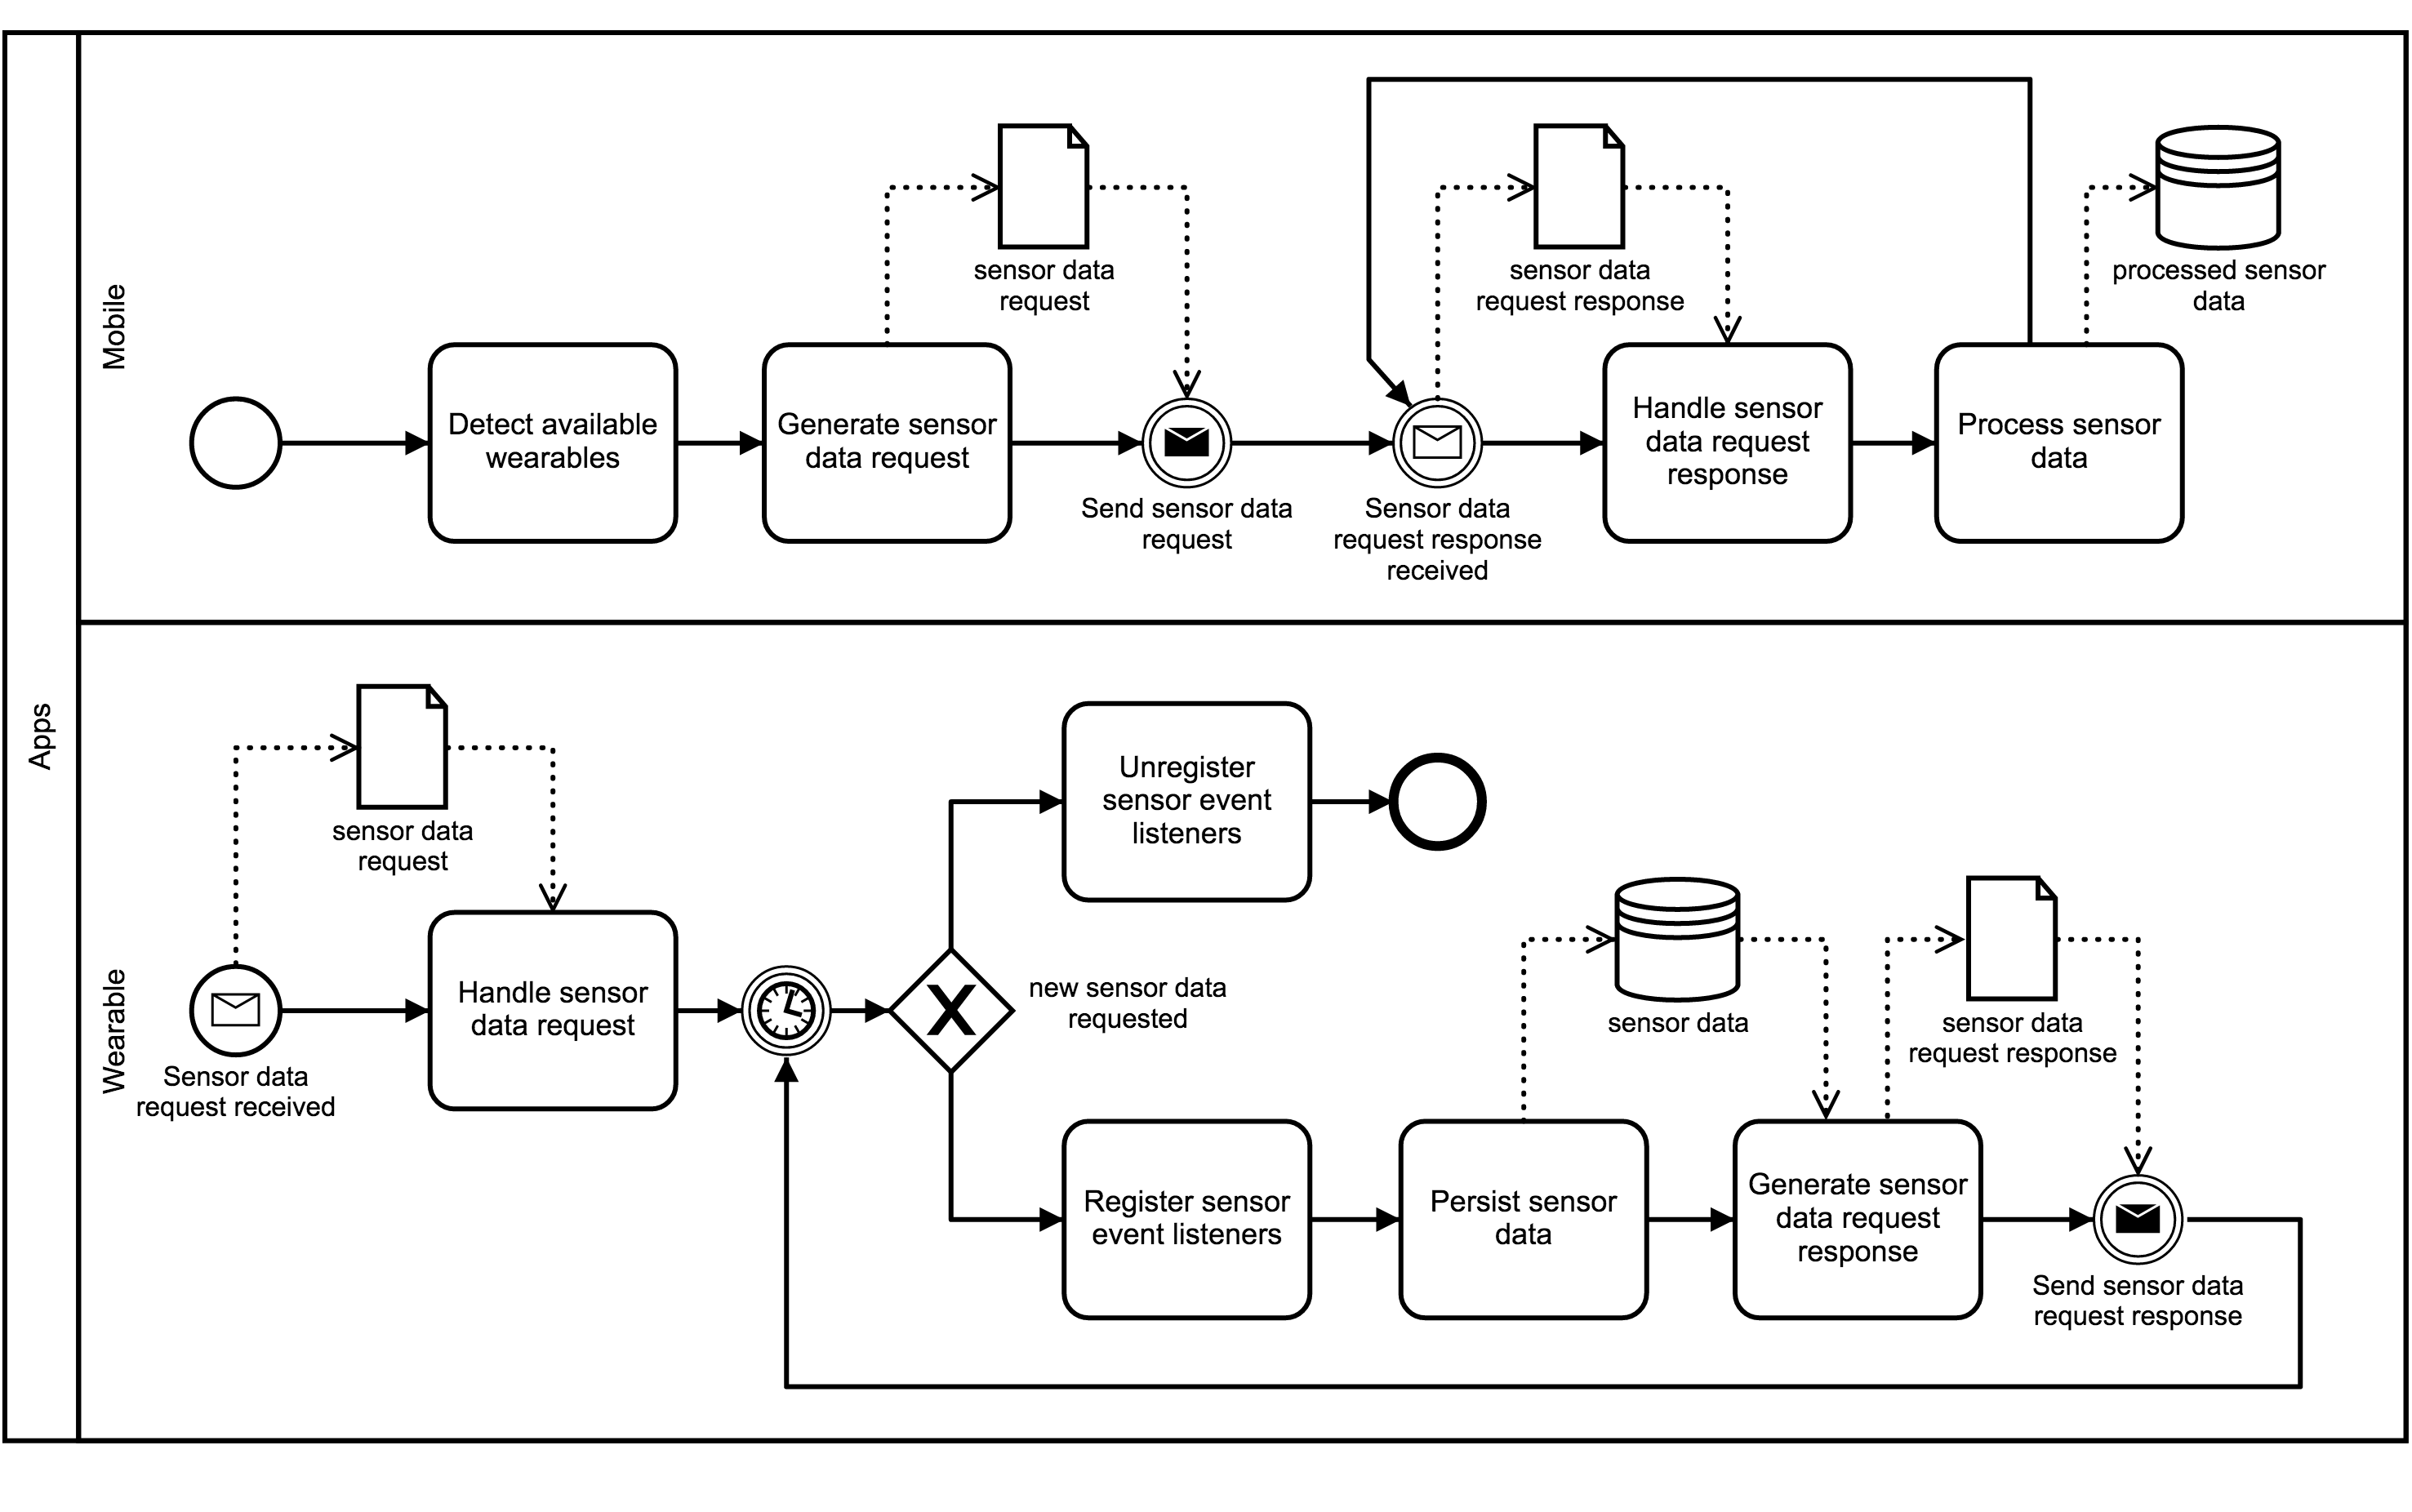
\includegraphics[width=\linewidth]{diagrams/apps.png}
	\caption[Caption for devices]{Wearable devices}
	\label{fig:devices}
\end{figure}

\subsection{Apple Watch}
While the currently available Apple Watches all provide sufficient hardware and enough sensors, the software does not allow 3rd party developers to take full advantage of this.
With WatchOS 2, Apple restricted apps running on the watch to only get access to sensor data while it's visible to the user.
For our project however, we needed a way to access sensor data from a background service, which simply isn't possible with the existing APIs.
Apple announced that in WatchOS 3 (which isn't available yet), this restriction will be eliminated. 

\subsection{UP by Jawbone}
\begin{itemize}[noitemsep]
	\item 2h API delay
	\item Can't provide required data frequency
\end{itemize}

\subsection{Microsoft Band}
\begin{itemize}[noitemsep]
	\item Awesome, but less users than competition
	\item Limited to SDK functionality
\end{itemize}

\subsection{Android Wear}
Android Wear is a platform for smartwatches that many devices from different manufacturers build upon.
Although it's customized to match the conditions of a watch, it's still a full Android OS without any limitations.
Because of Androids open nature, it's possible to use everything that the devices offer without any software restrictions.

\subsection{Decision}

Unlike the Apple Watch, Android Wear devices are able to connect to devices that don't belong to the same ecosystem, which increases the number of potential users. Although Apple topped Androids market share by almost 30\%\footnote{According to IDC Worldwide Quarterly Wearable Device Tracker} in 2015, we decided to develop for the Android platform because of the restrictions mentioned above.

\clearpage